\section{Why do NullPointerExceptions happen?}
\label{sec:why-do-nullp}

As you as you start playing with pointers to create dynamic data
structures you will soon receive a
\verb+NullPointerException+. Although we will learn more about
exceptions in the near future, a short explanation may be helpful
now. 

Java throws a \verb+NullPointerException+ when it tries to follow a
pointer and it cannot. This happens if the pointer is \verb+null+,
i.e.~it is not pointing anywhere. If it is not pointing anywhere, it
cannot be followed to any object. 

Let's see a small example. Imagine that you have two Strings in your
code: 

\begin{verbatim}
    String str1 = "This is a test string.";
    String str2 = null;
    println "First string's length: " + str1.length();
    println "Second string's length: " + str2.length();
\end{verbatim}

This code will compile without problems: it is syntactically
correct. However, when you execute the code you will get a
\verb+NullPointerException+: 

\begin{verbatim}
    First string's length: 22
    Exception in thread "main" java.lang.NullPointerException
         at MyClass.main(MyClass.java:15)
\end{verbatim}

This is because Java is trying to follow the pointer of \verb+str2+ to
execute the method \verb+length()+, but it is findind the pointer is
not pointing anywhere (Figure~\ref{fig:uilll}). 

\begin{figure}[htbp]
  \centering
  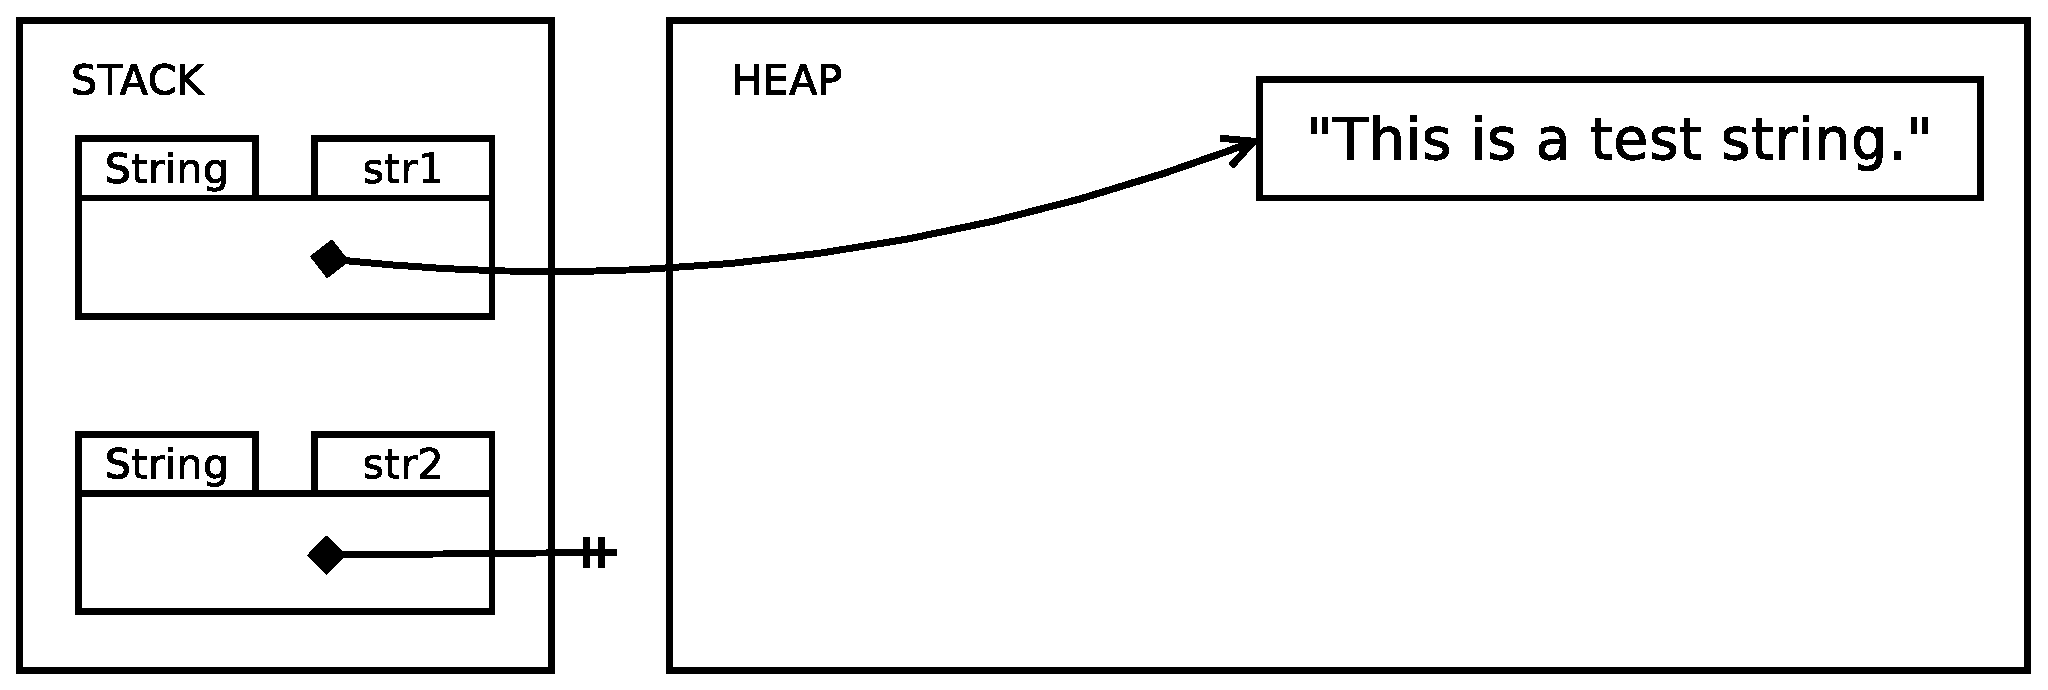
\includegraphics[width=\textwidth]{gfx/null-pointer-exception}
  \caption{If Java tries to follow a null pointer it throws a
    NullPointerException. In the example, this happens with String
    str2.} 
  \label{fig:uilll}
\end{figure}

\subsection{Is this a problem only for methods?}
\label{sec:this-problem-only}

We have said that member fields should be private, so at first sight
it may seem that a \verb+NullPointerException+ can only be the result
of calling a method on a null pointer, as in the example
above. Admittedly, this is the most common source of
\verb+NullPointerException+, but not the only one. 

Private member fields cannot be accessed from outside the class, but
they can be accessed in the class. You must keep in mind that the code
of a class is the same code for all objects of that class, so it may
be accessing member fields of more than one object. 

To illustrate the point, let's look at a possible implementation of
method \verb+equals+ of class \verb+String+: 

\begin{verbatim}
    /** 
     * Possible (non-real) implementation of String.equals().
     * Assumes class String contains an array of chars
     * called charArray.
     * 
     * The method is used like "str1.equals(str2)".
     */
    public boolean equals(String other) {
       if (this.length() != other.length()) {
          return false;
       }
       for (int i = 0; i < charArray.length; i++) {
          if (this.charArray[i] != other.charArray[i]) {
             return false;
          }
       } 
       return true;
    }
\end{verbatim}

This method seems quite clear. First, the lengths of the string where
the method is called 
(``this'', e.g. str1) and the other string (parameter ``other'',
e.g. str2) are compared in size. If they have different lengths they
are obviously different, so \verb+false+ is returned. If they have the
same length, they are compared character by character; as soon as a
character is different, \verb+false+ is returned. If the loop reached
the end, that means that all characters are equal, and \verb+true+ is
returned. 

Simple and clear, and it works\ldots or not. What happens if I compare
with a string where \verb+charArray+ is \verb+null+? I will get a
verb+NullPointerException+ when I try to access
\verb+other.charArray[i]+. This is a private field and it is accessed
from inside the class' code\ldots from another object. 

\subsection{What can I do about it?}
\label{sec:what-can-i}

In simple programs, like the ones we have done so far, it is easy to
keep track of all pointers to make sure they are not \verb+null+. Real
programs, on the other hand, have hundreds of classes containing
thousands of pointers. No human being can keep track of hundreds or
thousands of pieces of data: that is what computers where invented
for\footnote{Andrew Booth, founder of the Department of Computer
  Science at Birkbeck, invented one of the first computers to relieve
  his fellow crystallographers of the “tyranny of mathematics”,
  referring to how they had to perform heavy calculations involving a
  lot of numbers by hand.}.

But there is something that programmers \emph{can} do, and it checking
whether a pointer is null before following it. The method above would
be safer if written as follows: 

\begin{verbatim}
    /** 
     * Possible (non-real) implementation of String.equals().
     * Assumes class String contains an array of chars
     * called charArray.
     * 
     * The method is used like "str1.equals(str2)".
     */
    public boolean equals(String other) {
       if (other == null) {
          return false;
       }
       if (this.charArray == null || other.charArray == null) {
          return false;
       }
       if (this.length() != other.length()) {
          return false;
       }
       for (int i = 0; i < charArray.length; i++) {
          if (this.charArray[i] != other.charArray[i]) {
             return false;
          }
       } 
       return true;
    }
\end{verbatim}

As you can see, the first thing this method does is checking that the
argument is not null (``this'' string can never be null, otherwise the
method would not be in execution); if it is, it cannot be equal to
``this'' string so \verb+false+ is returned. The second thing is
checking that the arrays are not null; if any of they are, there is no
comparison possible and \verb+false+ is returned. From them on,
assured that all pointers are non-null, the method continues normally
as we have seen above. 

\subsection{Conclusion}
\label{sec:conclusion}

Null pointers are not pointing anywhere. Trying to access a field or a
method they are pointing to will result in a
\verb+NullPointerException+. We must be careful to prevent this from
happening in our code. 

Sometimes it is impossible to make sure whether a pointer is null or
not, e.g. when the program is very complex and has hundreds of
classes, or when we reuse code from another programmer. In those
cases, we must protect ourselves by checking that pointers are not
\verb+null+ before following them. 



%%% Local Variables:
%%% mode: latex
%%% TeX-master: "main"
%%% End:
